\subsection{Autoencoder}

Autoencoders are specific types of neural networks used to learn efficient encodings of unlabeled data and then decode them to reconstruct the original data \cite{10.5555/104279.104293, bank2021autoencoders}. Autoencoders can be represented by two models, the encoder $E_\phi$ and the decoder $D_\theta$, where $\phi$ and $\theta$ are the parameters of the model. The relationship between these can be formulated as such: 

\begin{equation}\label{eq:enc}
E_\phi: X \rightarrow Z 
\end{equation}
\begin{equation}\label{eq:dec}
D_\theta: Z \rightarrow X
\end{equation}

$E_\phi$ compresses data $X$ into a latent representation $Z$. $D_\theta$ then decodes $Z$, thus outputting a reconstructed dataset of the same dimensions as the input. $E_\phi$ can be seen as a compressing model, while $D_\theta$ can be seen as a decompressing model. This is further showcased in Figure \ref{fig:aediagram}. 

\begin{figure}[!h]
    \centering
    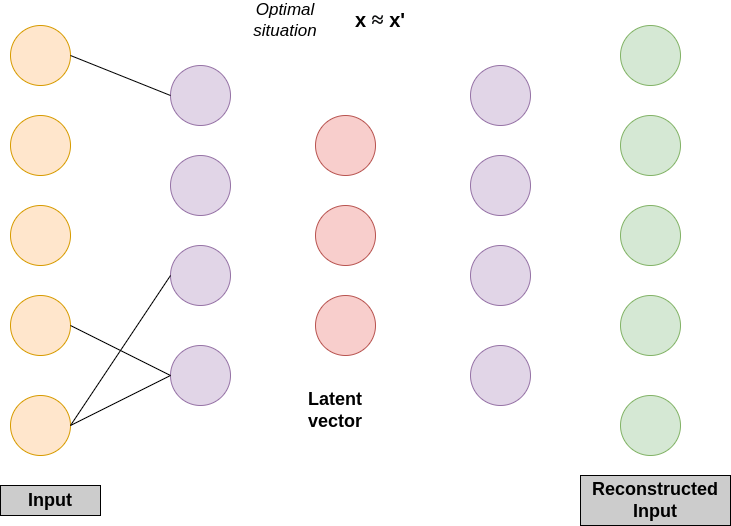
\includegraphics[scale=0.4]{figures/ae.png}
    \caption{Example of a dense autoencoder architecture}
    \label{fig:aediagram}
\end{figure}

The optima for any kind of autoencoder becomes that of lossless encoding, which can be described as such:
\begin{equation}
    X' \approx D_\theta(E_\phi(X))
\end{equation}

When the model is sufficiently trained for a specific task, $D$ \textit{may} become unnecessary for certain applications such as data reconstruction and denoising \cite{vincent2010stacked}. If the primary goal is feature extraction or dimensionality reduction, $E$ alone can be used to map input data to the lower-dimensional latent space. By utilizing only $E$, the overall complexity and size of the model $M$ can be reduced, which may be beneficial in scenarios with computational or memory constraints. For other tasks, including image reconstruction \cite{7797236}, signal analysis \cite{andrysiak2016machine}, and anomaly detection \cite{bank2021autoencoders}, the entire model is often needed.
\subsubsection{Latent Space}

The latent space $Z$ in autoencoders aims to capture essential features of the input data $X$ in a lower-dimensional representation, as displayed in Figure \ref{fig:aediagram}. However, traditional autoencoders face limitations in their generative capabilities \cite{bank2021autoencoders}. While they are trained to reconstruct original data accurately, they cannot typically generate new, diverse samples from $Z$. This limitation arises because regular autoencoders do not force any specific structure on $Z$ beyond compressing $X$. As a result, the latent representations may not be continuous or meaningful generative tasks.

\subsubsection{Limitations}
In addition to the issues with regular autoencoders in regard to decoding the latent space, these autoencoders have several disadvantages. The first of these is overfitting. Secondly, the lack \textit{regularization}, which can lead to poor generalization to unseen data. Furthermore, noise in the input data may potentially lead to large changes in the latent space. 

\subsubsection{Convolutional Autoencoders}
As mentioned in Section \ref{back:linear}, dense networks can struggle with feature extraction. This is also the case for dense autoencoders. By introducing convolutional layers, the autoencoder becomes more adept at image reconstruction and denoising \cite{zhang2018better}. These networks are called convolutional autoencoders (\acrshort{cae}). Another benefit of these are the reduction of parameters, as mentioned in Section \ref{back:cnn}.

